\documentclass[10pt]{article}
\usepackage{icmlko}

\icmlmeta{IP 파운데이션 월드모델}{340}{버릴 것이 없다}{계열 넷을 하나씩 빼 보니 다 벌고 있다 --- 그리고 그것이 어제의 이름을 고친다}

\begin{document}

\twocolumn[
\icmlheader

\begin{abstract}
노트 339가 무작위 열 하나에 판이 $-$0.1262 내려간다고 재고 \textbf{``축
스물셋 중 안 버는 것을 빼면 오른다''}를 갈래로 뒀다. 계열 넷을 하나씩
뺐다.

\begin{center}\footnotesize
\begin{tabular}{lrrrr}
\hline
뺀 것 & 축 & 판 차 & SD & 양수 \\
\hline
태그 & 6 & $-$0.0444 & 0.0089 & \textbf{0/12} \\
검색 & 3 & $-$0.0343 & 0.0072 & \textbf{0/12} \\
달력 & 6 & $-$0.0072 & 0.0065 & 2/12 \\
위키 & 3 & $-$0.0070 & 0.0058 & 1/12 \\
\hline
\end{tabular}
\end{center}

\textbf{넷 다 벌고 있다.} 태그와 검색은 크게($-$0.044 · $-$0.034 ·
둘 다 12/12 음수), 달력과 위키는 미결정 폭 안이지만 부호가 선다
(10/12 · 11/12). \textbf{버릴 계열이 없다.}

\textbf{그런데 이 수가 어제의 이름을 고친다.} 노트 338 · 339가 위약 열의
값을 \textbf{``열 하나의 값''}이라 불렀다. 그렇다면 실제 축 셋(검색)을
빼면 자리값 $3{\times}0.126 = +0.38$ 이 돌아오고 정보만 잃어야 한다.
\textbf{실제로는 $-$0.034 다.} 자리값이 있었다면 검색의 정보가
$+$0.41 이어야 하는데 그런 축은 이 판에 없다.

\textbf{그러므로 $-$0.126 은 자리값이 아니다.} 약한 축은 안 쓰이면
그만이고, \textbf{무작위 축은 틀린 쪽으로 가른다.} 둘은 다른 것이었다.
이름을 고친다 --- \textbf{``열값''이 아니라 ``잡음 축이 끼치는 해''}다.

\textbf{그리고 노트 335를 다시 읽는다.} 거기서 아이돌 앨범 축의
\emph{진짜} 값과 \emph{섞은} 값이 똑같이 $-$0.05 였다. 그때는 ``열이
하나 늘어서''로 읽었는데, 오늘 보면 \textbf{그 축이 잡음과 구별이 안
됐다}는 뜻이다 --- 반대로 위키 축 넷은 $+$0.074 로 확실히 정보였다.
\end{abstract}
]

\section{계열 넷}

\begin{center}\footnotesize
\begin{tabular}{lrl}
\hline
계열 & 축 & 무엇 \\
\hline
검색 & 3 & 네이버 데이터랩(노트 128) \\
달력 & 6 & 요일 · 연휴 간격(노트 130 · 213) \\
위키 & 3 & 위키백과 사전 조회수(노트 149) \\
태그 & 6 & 웹툰 큐레이션 태그 SVD(노트 255) \\
\hline
\end{tabular}
\end{center}

\begin{figure*}[t]
\centering
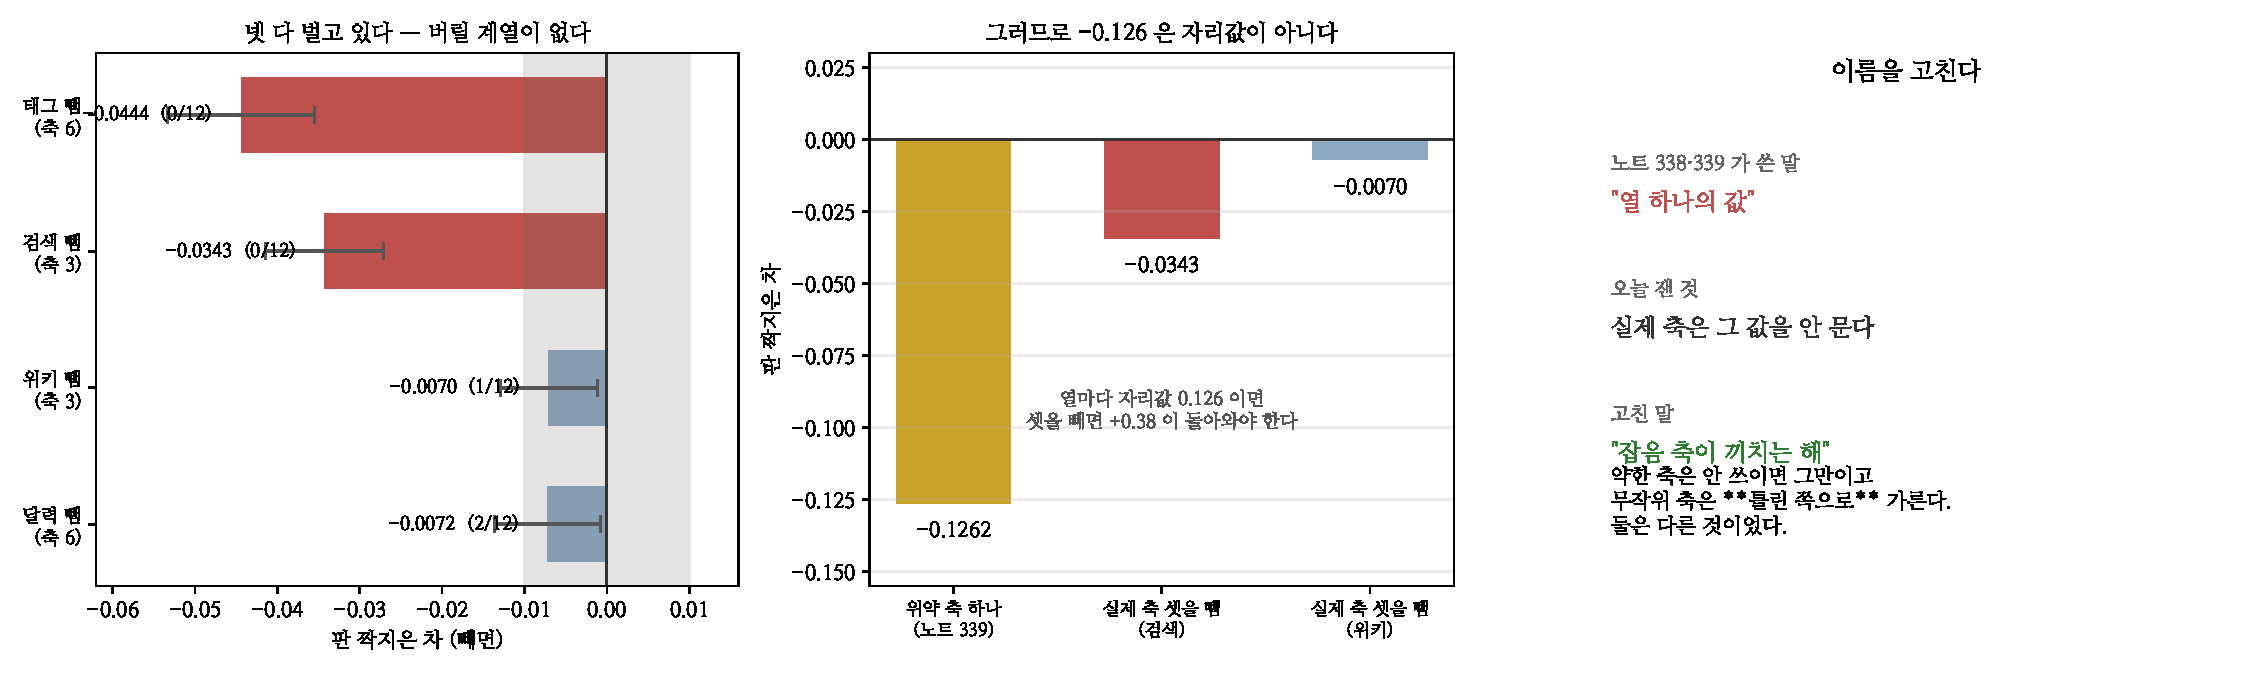
\includegraphics[width=\textwidth]{figs/prune.pdf}
\caption{왼쪽 --- 계열을 뺄 때. 가운데 --- 위약 값과 안 맞는다.
오른쪽 --- 이름을 고친다.}

\end{figure*}

\section{넷 다 벌고 있다}

태그가 제일 크다($-$0.0444) --- 웹툰 하나를 위해 만든 축인데 판을 그만큼
받치고 있다. 검색이 다음($-$0.0343). \textbf{달력과 위키는 미결정 폭
안이다}($-$0.0072 · $-$0.0070) --- 폭 규칙만 보면 빼도 되지만 부호가
10/12 · 11/12 로 서므로 \textbf{작지만 확실히 번다.}

\paragraph{그래서 안 뺀다} 이 실험실의 동점 처리는 ``$\rho$ 차가 짝지은
1 SE 안이면 좁은 쪽을 고른다''인데, 여기서는 차가 SD 보다 크다
($-$0.0072 대 0.0065). \textbf{동점이 아니다.}

\section{어제의 이름이 틀렸다}

\begin{center}\small
\begin{tabular}{lr}
\hline
위약 축 하나 더하기(노트 339) & $-$0.1262 \\
실제 축 셋 빼기(검색) & $-$0.0343 \\
실제 축 셋 빼기(위키) & $-$0.0070 \\
\hline
\end{tabular}
\end{center}

\textbf{열마다 $-$0.126 짜리 자리값이 있다면} 검색 셋을 뺄 때
$+$0.38 이 돌아오고 정보만 나가야 한다. 관측은 $-$0.034 다.
\textbf{산수가 안 맞는다.}

맞는 읽기는 이렇다 --- \textbf{나무는 쓸모없는 열을 그냥 안 쓴다.}
그런데 \emph{무작위} 열은 학습 잡음에 우연히 맞는 갈림을 준다. 그래서
붙이면 해롭고 빼면 회복되지만, \textbf{원래 있던 약한 축은 그런 갈림을
안 만든다}(만들었으면 이미 판이 낮았을 것이다).

\begin{center}\footnotesize
\begin{tabular}{ll}
\hline
약한 축 & 안 쓰인다 --- 값이 0 에 가깝다 \\
\textbf{잡음 축} & \textbf{틀린 쪽으로 가른다 --- $-$0.126} \\
\hline
\end{tabular}
\end{center}

\section{노트 335를 다시 읽는다}

\begin{center}\footnotesize
\begin{tabular}{lrl}
\hline
아이돌에 붙인 것 & 짝지은 차 & 다시 읽으면 \\
\hline
앨범 축(진짜) & $-$0.046 & \\
앨범 축(섞음) & $-$0.058 & \textbf{둘이 같다} \\
위키 축 넷 & $+$0.074 & 확실히 정보 \\
\hline
\end{tabular}
\end{center}

\textbf{앨범 축은 잡음과 구별이 안 됐다.} 학습에서 값$\sim$라벨이
$+$0.542 였는데도 그렇다 --- 노트 335가 이미 ``검사는 축이 무엇을 아는가를
재는데 비용은 그와 무관하다''고 적었고, 오늘 그 문장의 뒷부분이
\textbf{``유보에서 그 앎이 살아남는가''}로 바뀐다.

\section{남은 것}
\begin{center}\footnotesize
\begin{tabular}{ll}
\hline
갈래 & 왜 \\
\hline
\textbf{잡음 축 검사를 도구로} & 붙이기 전에 섞어서 견줘라 \\
축 하나씩 빼 보기 & 계열이 아니라 축 스물셋 \\
F6 · F10 도 잡음에 약한가 & 나무만의 병인가 \\
태그가 왜 $-$0.044 인가 & 웹툰용인데 판을 받친다 \\
\hline
\end{tabular}
\end{center}

\paragraph{규약} \textbf{두 노트 만에 이름을 고쳤다.} 노트 338이 ``열값
$-$0.09'', 노트 339가 ``열값 $-$0.126''이라 쓰고 값표까지 만들었는데,
오늘 실제 축을 빼 보니 그 값이 실제 축에는 안 붙는다. \textbf{위약으로
잰 것을 ``열의 값''이라 부른 것이 성급했다} --- 위약은 \emph{정보가 없는}
열이 아니라 \emph{틀리게 가르는} 열이었다. \textbf{위약이 재는 것이
무엇인지 위약만 보고는 모른다} --- 반대쪽(진짜를 빼기)을 같이 재야 갈린다.

\end{document}
